
\begin{figure}[t]

\begin{lstlisting}[mathescape=true,showlines=true]
void dijkstra (int **g, int src, int *dist,
               int *prev, int size, int inf {
$\color{OliveGreen}//~\braces{\p{AdjMat}(\texttt{g},\gamma) *
\mathsf{array}(\texttt{dist}, \_) * \mathsf{array}(\texttt{prev}, \_)}$
 Item* temp = (Item*) mallocN(sizeof(Item));
 int* keys = mallocN (size * sizeof (int));
 PQ* pq = pq_make(size); int i, j, u, cost;
 for (i = 0; i < size; i++)
 { dist[i] = inf; prev[i] = inf; keys[i] = pq_push(pq,inf,i); } $\label{code:assigninf}$
 dist[src]= 0; prev[src]= src; pq_edit_priority(pq,keys[src],0);
 while (pq_size(pq) > 0) {
$\color{OliveGreen}//~\braces{{\color{red}\exists \m{dist}, \m{prev}, \m{popped}, \m{heap}}.~\p{AdjMat}(\texttt{g},\gamma) * {\color{red}\p{PQ}(\texttt{pq},\m{heap})} *
{\color{red}\mathsf{Item}(\texttt{temp}, \_)} * \null \\
\mathsf{array}(\texttt{dist},{\color{red}\m{dist}}) *
\mathsf{array}(\texttt{prev}, {\color{red}\m{prev}}) *
{\color{red}\mathsf{array}(\texttt{keys}, \m{keys}}) /| \null \\
{\color{red}\m{linked\_correctly}(\gamma, \m{heap}, \m{keys}, \m{dist}, \m{popped})} /| \null \\
{\color{red}\m{dijk\_correct}(\gamma,\texttt{src},\m{popped},\m{prev},\m{dist})}}$ $\label{code:whileinv}$
  pq_pop(pq, temp); u = temp->data; $\label{code:pop}$
  for (i = 0; i < size; i++) {
$\color{OliveGreen}//~\braces{{\color{red}\exists \m{dist'}, \m{prev'}, \m{heap'}}.~\p{AdjMat}(\texttt{g},\gamma) * \p{PQ}(\texttt{pq},{\color{red}\m{heap'}}) * \null \\
\mathsf{array}(\texttt{dist},\m{\color{red}dist'}) *
\mathsf{array}(\texttt{prev}, \m{\color{red}prev'}) *
\mathsf{array}(\texttt{keys}, \m{keys}) * \null \\
\mathsf{Item}(\texttt{temp}, \m{\color{red}(\texttt{keys[u]}, \texttt{dist[u]}, \texttt{u})}) /|
\m{\color{red}min(\texttt{dist[u]}, \m{heap'})} /| \null \\
{\m{linked\_correctly}(\gamma, \m{\color{red}heap'}, \m{keys}, \m{\color{red}dist'},
{\color{red}\m{popped} \uplus \{\texttt{u}\}})} /| \null \\
{\color{red}\m{dijk\_correct\_weak}({\color{OliveGreen}\gamma, \texttt{src}}, \m{popped} \uplus \{\texttt{u}\}, \m{prev'}, \m{dist'}, \texttt{i}, \texttt{u})}}$ $\label{code:forinv}$
   cost = getCell(g, u, i); $\label{code:cost}$
   if (cost < inf) {
    if (dist[i] > dist[u] + cost) { $\label{code:overflow}$
     dist[i] = dist[u] + cost; prev[i] = u; $\label{code:update1}$
     pq_edit_priority(pq, keys[i], dist[i]); $\label{code:update2}$
  }}}} $\color{OliveGreen}//~\braces{{\color{red}\exists \m{dist''}, \m{prev''}}.~\p{AdjMat}(\texttt{g},\gamma) * \p{PQ}(\texttt{pq},\m{\color{red}\emptyset}) * {\mathsf{Item}(\texttt{temp}, {\color{red}\_})} * \null \\
 \mathsf{array}(\texttt{dist},\m{\color{red}dist''}) *
 \mathsf{array}(\texttt{prev}, \m{\color{red}prev''}) *
 \mathsf{array}(\texttt{keys}, \m{keys}) /| \null \\
{\color{red}\forall \m{dst}.~0 \le \m{dst} < \texttt{size} -> \m{inv\_popped}}(\gamma, \m{src}, {\color{red}\m{\gamma.V}, \m{prev''}, \m{dist''}, \m{dst}})}$ $\label{code:end}$
 freeN (temp); pq_free (pq); freeN (keys); return; }
\end{lstlisting}
\vspace{-1em}
\caption{C code and proof sketch for Dijkstra's Algorithm.}
\vspace{-1em}
\label{fig:decorated}
\end{figure}



\hide{
$\color{OliveGreen}//~\braces{{\color{red}\exists \m{dist''}, \m{prev''},\m{heap''}}.~\p{AdjMat}(\texttt{g},\gamma) * \p{PQ}(\texttt{pq},\m{\color{red}heap''}) *
  \mathsf{array}(\texttt{dist},\m{\color{red}dist''}) * \null \\
  \mathsf{array}(\texttt{prev}, \m{\color{red}prev''}) *
  \mathsf{array}(\texttt{keys}, \m{keys}) *
  \mathsf{Item}(\texttt{temp}, \m{(\texttt{keys[u]}, \texttt{dist[u]}, \texttt{u})} /| \null \\
  \m{min(\texttt{dist[u]}, \m{heap'})} /|
  {\color{red}\m{heap''} = \m{heap'} [\texttt{keys[i]} \mapsto (\texttt{dist[i]},\texttt{i})]} /| \null \\
  {\m{\color{red}dijk\_correct}(\gamma, \texttt{src}, \m{popped'}, \m{\color{red}prev''}, \m{\color{red}dist''})}}$ $\label{code:caughtup}$
}

\vspace{-0.75em}

Figure~\ref{fig:decorated} shows the code and proof
sketch of Dijkstra's algorithm.  Our code is implemented exactly
as suggested by CLRS~\cite{clrs} so we refer readers there for a
general discussion of the algorithm.
The adjacency-matrix-represented graph~$\gamma$ of \texttt{SIZE} vertices
is passed as the parameter \texttt{graph} along with the source vertex \texttt{src}
and two allocated arrays \texttt{dist} and \texttt{prev}.
The spatial predicate $\mathsf{array}(x,\vec{v})$ connecting an array pointer $x$ with its contents $\vec{v}$ is standard and unexciting.
Our spatial graph predicate is more interesting, in
that it nests arrays and connects the concrete memory values to an abstract mathematical
graph~$\gamma$, which in turn exposes an interface in the language of graph theory
(vertices, edges, labels, etc.).
\vspace{-0.5em}
\begin{equation*}
\begin{split}
\m{list\_addr} ((\m{block}, \m{offset}), \m{index}) &\defeq
  (\m{block}, \m{offset} + (\m{index} \times \texttt{sizeof}(\texttt{int}) \times \texttt{SIZE})) \\
\p{list\_rep}(\gamma, \m{i}, \m{base\_ptr}) &\defeq \mathsf{array}(\mathsf{graph2matrix}(\gamma)[\m{i}], \m{list\_addr}(\m{base\_ptr}, \m{i})) \\
\vspace{1em}
\p{graph\_rep}(\gamma, \m{g\_addr}) &\defeq \underset{\m{v} \in \gamma}{\bigstar} \m{v}  \mapsto\p{list\_rep}(\gamma, \m{v}, \m{g\_addr})
\end{split}
\end{equation*}
In general, these spatial representations are simple enough that they pose no special
challenge in the proof. Therefore, in our discussion below, we will not focus on 
issues such as making sure an array dereference is in bounds.

\note[new text]{
Dijkstra's algorithm uses a priority queue to greedily choose the 
next-cheapest unexamined vertex, as in line~\ref{code:pop}. Of course, the 
best-known distances to vertices are expected to improve as the algorithm
proceeds, and such improvements need to be logged in the PQ. 
In other words, Dijkstra's PQ needs to support the relatively nonstandard 
\texttt{decrease\_key} operation, which can be implemented in $\bigO(\log n)$ time
after a nontrivial amount of additional bookkeeping. One of our 
contributions is a verified binary heap-based PQ that supports \texttt{decrease\_key}.

Some implementations of Dijkstra \cite{blah, blah, blah} 
get by with a simpler PQ (or even without a PQ) by leveraging the fact that
the \texttt{dist} array already tracks the best-known cost to any vertex 
(see line~\ref{code:update1}). Such implementations maintain a list of 
examined vertices, and, when looking for the next-cheapest unexamined
vertex, simply scan \texttt{dist} for the cheapest vertex that has not
been examined. This is neat, but drags down performance unacceptably.
% each \texttt{pop\_min} now takes $\bigO(n)$ time.


} % end of note

With an approproate priority queue in hand, 
the key to the verification is the pure part of the loop
invariants on lines~\ref{code:whileinv} and~\ref{code:forinv}.  The \texttt{while} invariant $\m{dijk\_correct}(\gamma, \texttt{src}, \m{prev}, \m{dist}, \m{priq})$ has three parts:
\[
\begin{array}{l}
\forall \m{dst}.~\texttt{0} \le \m{dst} < \texttt{SIZE} -> \m{inv\_popped}(\gamma, \texttt{src}, \m{prev}, \m{dist}, \m{priq}, \m{dst}) /| \null \\
\hspace{11em}\m{inv\_unpopped}(\gamma, \texttt{src}, \m{prev}, \m{dist}, \m{priq}, \m{dst}) /| \null \\
\hspace{11em}\m{inv\_unseen}(\gamma, \m{prev}, \m{dist}, \m{priq}, \m{dst})
\end{array}
\]
A destination vertex $\m{dst}$ falls into one of three
categories:
\begin{enumerate}
\item $\m{inv\_popped}$: $\m{dst}$ has been fully processed, and has been
popped from the priority queue.
A globally optimal path from $\texttt{src}$
to $\m{dst}$ exists, the cost of this path is logged in
the \texttt{dist} array, and all the vertices visited by the path are also popped.
Further, the links of this path are logged in the \texttt{prev} array.
\item $\m{inv\_unpopped}$: $\m{dst}$ is reachable in
one hop from a popped ``\emph{mom}'' vertex.
This route is locally optimal: we cannot
improve the cost with a \emph{different} popped vertex.
The \texttt{prev} array logs
\emph{mom} as the best-known way to reach $\m{dst}$, and the \texttt{dist}
array logs the path cost via \emph{mom} as the best-known cost.
\item $\m{inv\_unseen}$: no path is currently known from $\texttt{src}$ to $\m{dst}$.
\end{enumerate}
After popping the lowest-cost vertex in line~\ref{code:pop}, we reach the invariant of
the \texttt{for} loop $\m{dijk\_correct\_weak}(\gamma, \texttt{src}, \m{prev}, \m{dist}, \m{priq}, \texttt{i}, \texttt{u})$:
\[
\begin{array}{l}
\forall \m{dst}.~\texttt{0} \le \m{dst} < \texttt{SIZE} -> \m{inv\_popped}(\gamma, \m{src}, \m{prev}, \m{dist}, \m{priq}, \m{dst}) /| \null \\
\hspace{11em}\m{inv\_unseen}(\gamma, \m{prev}, \m{dist}, \m{priq}, \m{dst}) /| \null \\
\forall \m{dst}.~\texttt{0} \le \m{dst} < \texttt{i} -> \m{inv\_unpopped}(\gamma, \m{src}, \m{prev}, \m{dist}, \m{priq}, \m{dst}) /| \null \\
\forall \m{dst}.~\texttt{i} \le \m{dst} < \texttt{SIZE} -> \m{inv\_unpopped\_weak}(\gamma, \m{src}, \m{prev}, \m{dist}, \m{priq}, \m{dst}, \texttt{u})
\end{array}
\]
We now have four cases, many of which are familiar from $\m{dijk\_correct}$:
\begin{enumerate}
\item $\m{inv\_popped}$: $\m{dst}$ has been fully processed, and has been
popped from the priority queue.  For all popped vertices \emph{except for} \texttt{u},
this is trivial from $\m{dijk\_correct}$. For \texttt{u} itself, we reach the heart of Dijkstra's correctness: the cost to the fringe vertex with minimum cost cannot be further improved.  %The associated entailment is not trivial.
\item $\m{inv\_unseen}$: no path is known from $\texttt{src}$ to $\m{dst}$.  This is straightforward.
\item $\m{inv\_unpopped}$ (less than \texttt{i}): $\m{dst}$ is reachable in
one hop from a ``\emph{mom}'' vertex, which is itself popped.  Initially this is trivial since $\texttt{i}=0$, and we restore it as \texttt{i} climbs by updating costs when they can be improved, as in lines~\ref{code:update1}~and~\ref{code:update2}.
\item $\m{inv\_unpopped\_weak}$ (between than \texttt{i} and \texttt{SIZE}):
$\m{dst}$ is reachable in one hop from a popped ``\emph{mom}'' vertex.
However, the path to $\m{dst}$ specifically \emph{does not go via} \texttt{u}.
%This is fairly intuitive, since the for loop has not yet repaired $\m{dst}$.
This fact is key to restoring $\m{inv\_unpopped}$ as $\texttt{i}$
increments.
\end{enumerate}
The formal definitions for the above predicates can be found in the Appendix.
%, and the key subdefinitions upon which they rely, 

At the end of the \texttt{for} loop, the fourth case will fall away (\texttt{i = SIZE}),
allowing us to infer the \texttt{while} invariant $\m{dijk\_correct}$ from $\m{dijk\_correct\_weak}$ and thus continue the \texttt{while} loop.
The while loop will break precisely when no item in the priority queue has cost
less than \texttt{INF}. The second clause of the \texttt{while} loop invariant
$\m{dijk\_correct}$ then falls away: all reachable vertices have been optimized,
and the rest are unreachable altogether. We are done.

\hide{

While loop's invariant, which is stated on line
and explained further in Figure~\ref{fig:defns}.


This three-part invariant is trivially true before the while loop.
On line~\ref{code:pop}, the minimal vertex from the priority queue is popped,
thus breaking the invariant.

First, we must show that the minimal vertex $\m{u}$
obeys $\m{inv\_popped}$. \emph{i.e.}, show that the locally
optimal path to $\m{u}$ is, in fact, globally optimal.
This comes from blah blah blah

\newcommand{\s}{11}
\begin{figure}[htbp]
  \centering
  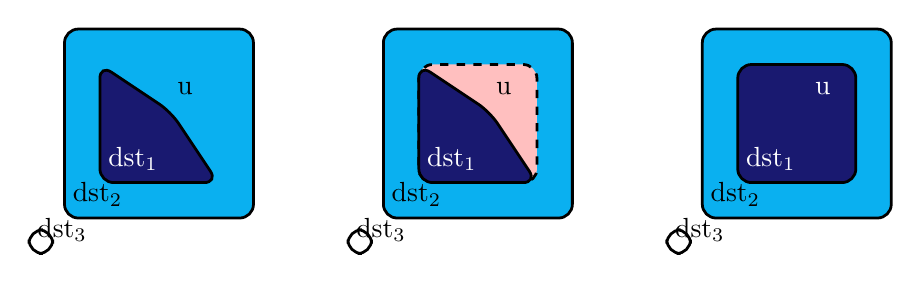
\begin{tikzpicture}[x=0.3cm, y=0.3cm,
      popped/.style={rounded corners=5pt, line width=1pt, draw, fill=MidnightBlue},
      fringe/.style={rounded corners=5pt, line width=1pt, draw, fill=ProcessBlue},
      popping/.style={rounded corners=5pt, line width=1pt, draw, dashed, fill=pink},
      unseen/.style={rounded corners=5pt, line width=1pt, draw}]
    \draw[unseen] (0,0) -- (\s,0) -- (\s,\s) -- (0,\s) -- cycle;
    \draw[fringe] (1.5,1.5) -- (9.5,1.5) -- (9.5,9.5) -- (1.5,9.5) -- cycle;
    \draw[popped] (3,3) -- (8,3) -- (6,6) -- (3,8) -- cycle;
    \node at (1.4,1) {dst$_3$};
    \node at (2.9,2.5) {dst$_2$};
    \node at (4.4,4) {\color{white}dst$_1$};
    \node at (6.6,7) {u};
    \tikzset{shift={(13.5,0)}}

    \draw[unseen] (0,0) -- (\s,0) -- (\s,\s) -- (0,\s) -- cycle;
    \draw[fringe] (1.5,1.5) -- (9.5,1.5) -- (9.5,9.5) -- (1.5,9.5) -- cycle;
    \draw[popping] (3,3) -- (8,3) -- (8,8) -- (3,8) -- cycle;
    \draw[popped] (3,3) -- (8,3) -- (6,6) -- (3,8) -- cycle;
    \node at (1.4,1) {dst$_3$};
    \node at (2.9,2.5) {dst$_2$};
    \node at (4.4,4) {\color{white}dst$_1$};
    \node at (6.6,7) {u};

    \tikzset{shift={(13.5,0)}}

    \draw[unseen] (0,0) -- (\s,0) -- (\s,\s) -- (0,\s) -- cycle;
    \draw[fringe] (1.5,1.5) -- (9.5,1.5) -- (9.5,9.5) -- (1.5,9.5) -- cycle;
    \draw[popped] (3,3) -- (8,3) -- (8,8) -- (3,8) -- cycle;
    \node at (1.4,1) {dst$_3$};
    \node at (2.9,2.5) {dst$_2$};
    \node at (4.4,4) {\color{white}dst$_1$};
    \node at (6.6,7) {\color{white}u};
  \end{tikzpicture}
  \caption{Popping $\m{u}$}
\end{figure}

Next, we must account for the ripple effect that popping
$\m{u}$ could have had on the other vertices.
In particular, it is possible that a vertex obeying $\m{inv\_unpopped}$ can
improve its cost via $\m{u}$, and that an unreachable vertex
obeying $\m{inv\_unseen}$ can now be reached via $\m{u}$.
The for loop repairs these breakages by
checking if a path via $\m{u}$ is an improvement for such vertices, and, if so,
edits both arrays and the priority queue as seen on line~\ref{code:update}.

The for loop's invariant is similar to that of the while loop---$\m{inv\_unseen}$
and $\m{inv\_popped}$ are preserved as-is, modulo the popping of
$\m{u}$ as discussed above. The key edit is in $\m{inv\_unpopped}$. blah blah blah

}



